\documentclass{article}

\usepackage[T1]{fontenc}
\usepackage[utf8]{inputenc}
\usepackage{mdwlist} % To have compact lists
\usepackage{hyperref} % To have links to URLs
\usepackage{float} % To force images to the right place
\usepackage{listings} % To display source code

\usepackage{caption}
\usepackage{subcaption}

% To include images
\usepackage{graphicx} 
\graphicspath{ {images/} } % location of images

% Disables automatic indents globally
%\setlength{\parindent}{0pt}


\begin{document}

% - - - - Header Begins - - - -
\begin{center}
	{\LARGE \textbf{Project Plan}} \\
	\vspace{0.5em}
	\textsl{Team $\lambda$ Lovelace}
\end{center}

\vspace{0.5em}

\begin{center}
	10th June 2016 \\
	COMP47250, Team Software Project 2016 \\ 
	University College Dublin, Ireland \\
\end{center}

\vspace{0.5em}
% - - - - Header Ends - - - -


\noindent This is a project plan for the team $\lambda$ Lovelace, summer 2016. The module formally started 2016.05.16 and will end in a final submission 2016.08.19. Four weeks have passed when this document was submitted. 


\section{Vision}
% 300 words approx.
% A clear description of the overall vision for your project
% 
% What are you doing?
% Why are you doing it?
% Who will use it?
% How will they use it?

Our project is to create a collaborative recommender system for tweets; a more personalised tweet stream.


\section{Minimum Viable Product}
% 500 words approx.
% A description of your first minimal viable product including what you will learn from deploying this and what you would measure in order to learn it. (Even if you are not taking a lean approach to managing your project you should be able to articulate an MVP.)
% 
% + How will you build your system? (System Diagram)
% 		- Front-end: user interface components
%		- Back-end technical components
%		- Data sources: What data will you use and how will you access it?
%	+ How will you evaluate your system? (Initial ideas)

Text


\section{Project Management}
% 200 words approx.
% How will you run your project?
From the start we have been working together around a ring table in room B1.06 in the computer science building at UCD. We follow a flexitime schedule but aim to work together from 10:00 - 18:00 every week day. We do not work over weekends but if a team member needs to take a weekday off he or she tries to catch up on weekends so we all put in roughly the same amount of hours.
\\\\
For source control we use Git in a private repository on GitHub. It should be noted that each team was allocated a repository in the organisation \linebreak \mbox{\textit{ucd-nlmsc-teamproject}} \cite{ucdgithub}. We however created our own repository \cite{gitrepo} so we could have unrestrained access to third party tools that required \textit{owner} rights\footnote{we were granted \textit{admin} rights but for some tools it's not enough}.
\\\\
For external communication we use a group conversation on Facebook Messenger. We tried chat with Slack  but favoured Messenger for simplicity. Slack now serves mostly as a notification hub for GitHub issues, commits, pull requests, etc.
\\\\
For project management we use ZenHub \cite{zenhub}. It's a Chrome browser extension that `hijacks' the GitHub website and augments it with extra features. The features we primarily use:

\begin{samepage}
\begin{itemize*}
	\item Kanban style board to have an overview of issues
	\item Story points for issue effort estimations
	\item Burndown charts for milestones
\end{itemize*}
\end{samepage}


\begin{figure}[H]
    \centering
    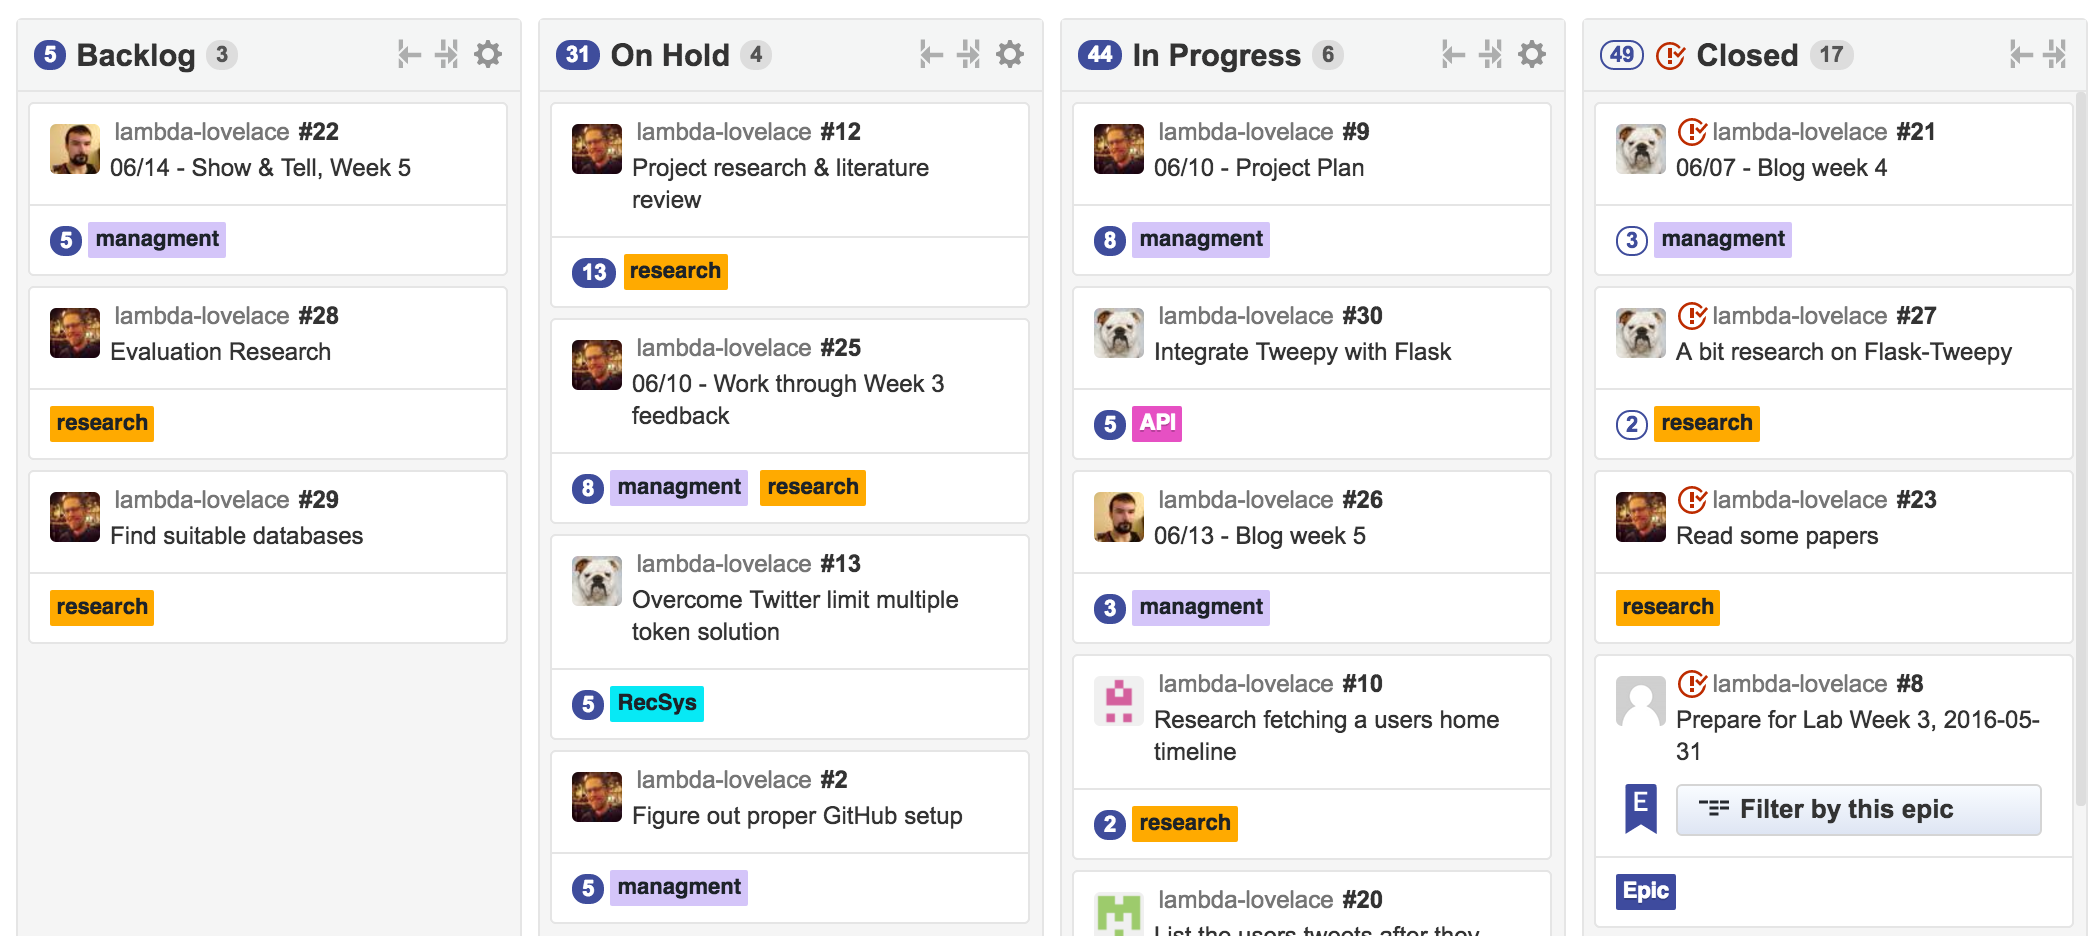
\includegraphics[width=0.8\textwidth]{kanbanboard}  
    \caption{Screenshot from our Kanban board that ZenHub provides}
\end{figure}

\begin{figure}[H]
    \centering
    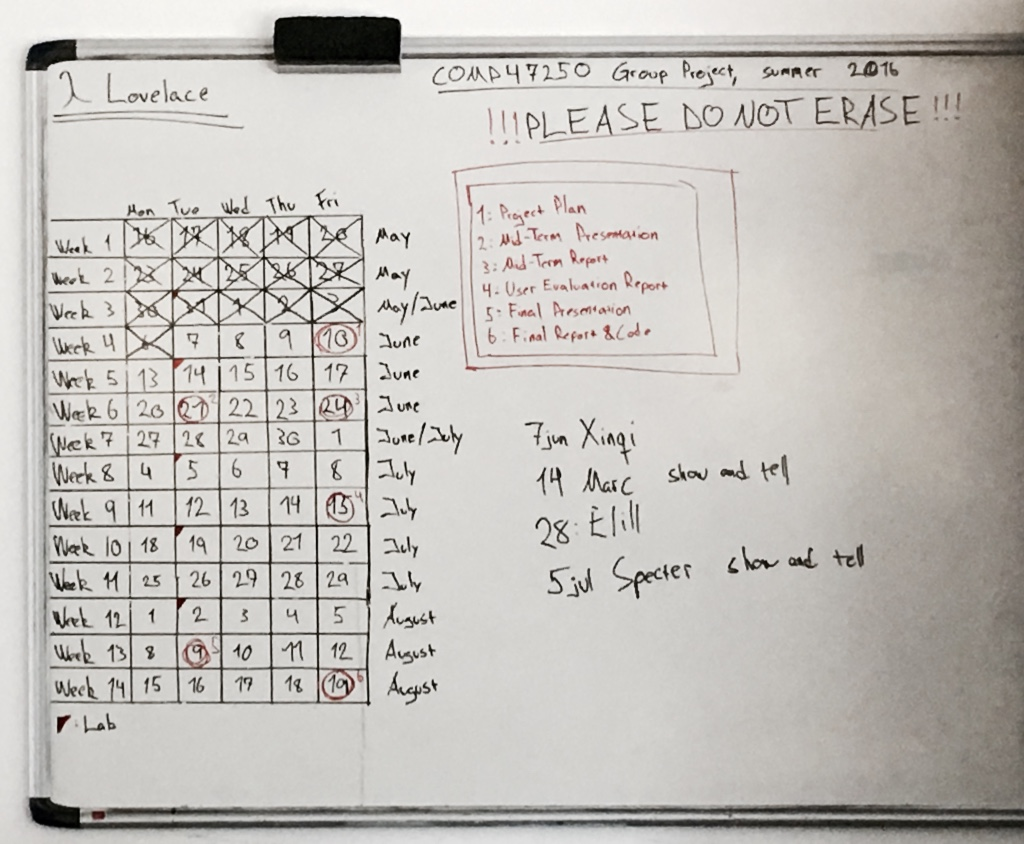
\includegraphics[width=0.8\textwidth]{whiteboard}    
    \caption{A picture of our time schedule whiteboard}
\end{figure}


\section*{Other}

\begin{samepage}
\begin{center}
\begin{minipage}[t]{.4\textwidth}
	\textbf{Students}:
		\begin{itemize*}
			\item Xinqi Li
			\item Marc Laffan
			\item Junyang Ma
			\item Jón Rúnar Helgason
			\item Eazhilarasi Manivannan
		\end{itemize*}
\end{minipage}
~
\begin{minipage}[t]{.4\textwidth}
	\textbf{Module co-ordinators}:
	\begin{itemize*}
		\item Georgiana Ifrim
		\item Brian Mac Namee
		\item Derek Greene
	\end{itemize*}
\end{minipage}
\end{center}
\end{samepage}

\vspace{0.5em}

\begin{thebibliography}{9} 

\bibitem {vaki}
	$\lambda$ Lovelace blog, \url{http://jonrh.github.io/lambda-lovelace/}
	
\bibitem {ucdgithub}
	Negotiated Learning Project organisation on GitHub \\
	\url{https://github.com/ucd-nlmsc-teamproject}

\bibitem {gitrepo}
	$\lambda$ Lovelace code repository on GitHub \\
	\url{https://github.com/jonrh/lambda-lovelace/}
	
\bibitem {zenhub}
	ZenHub official website \url{https://www.zenhub.com/}


\end{thebibliography}



\end{document}